%%%%%%%%%%%%%%%%%%%%%%%%%%%%%%%%%%%%%%%%%%%%%%%%%%%%%%%%%%%%%%%%%%%%%%
% Lớp 10 | Phương pháp tọa độ trong mặt phẳng (𝑂𝑥𝑦) | Đường thẳng trong mặt phẳng tọa độ
% Dạng 0H9?3-5: Bài toán về khoảng cách
% Số câu: 29  (sinh tự động bởi tach_cau.py; từ nay thầy sửa trực tiếp file này)
%%%%%%%%%%%%%%%%%%%%%%%%%%%%%%%%%%%%%%%%%%%%%%%%%%%%%%%%%%%%%%%%%%%%%%

%%%%%%%%%%%%%%%% TRẮC NGHIỆM 4 PHƯƠNG ÁN %%%%%%%%%%%%%%%%

% nguồn: MaHoaNH_TracNghiem_Lop10
\begin{ex}%[0H9N3-5]%[ma:1e072ad2]
	Khoảng cách từ điểm $M(1; 2)$ đến đường thẳng $\Delta\colon  3x+4y-3=0$ bằng
	 \choice
		{\True  $\dfrac{8}{5}$}
		{$\dfrac{5}{8}$} 
		 {$\dfrac{7}{5}$}
		 {$8$}
	\loigiai{ 
		Ta  có $\mathrm{d}(M;(\Delta))=\dfrac{|3\cdot 1+4\cdot2-3|}{\sqrt{3^2+4^2}}=\dfrac{8}{5}$.
	 }
\end{ex}

% nguồn: MaHoaNH_TracNghiem_Lop10
\begin{ex}%[0H9N3-5]%[ma:3fd26717]
	Trong mặt phẳng toạ độ  $Oxy$, khoảng cách từ điểm $A(1;5)$ đến đường thẳng $\Delta \colon x+y-3=0$ là
	 \choice
		{$\dfrac{1}{\sqrt{2}}$} 
		 {$1$}
		{$\sqrt{2}$} 
		 {\True $\dfrac{3}{\sqrt{2}}$}
	\loigiai{ 
		 Ta có $\mathrm{d}(A,\Delta)=\dfrac{|1+5-3|}{\sqrt{1^2+1^2}}=\dfrac{3}{\sqrt{2}}$.
	} 
\end{ex}

% nguồn: MaHoaNH_TracNghiem_Lop10
\begin{ex}%[0H9N3-5]%[ma:8fd15d08]
	Trong mặt phẳng tọa độ $Oxy$, cho  đường thẳng $\Delta\colon 3x+4y+5=0$. Khoảng cách từ gốc tọa độ đến đường thẳng $\Delta$ bằng
	 \choice
		{$2$} 
		{\True $1$} 
		{$3$} 
		 {$4$}
	\loigiai{ 
		Khoảng cách từ gốc  tọa độ đến đường thẳng $\Delta$ là\\
		 \centerline{$\mathrm{d}(O; \Delta)=\dfrac{|3\cdot 0 +4\cdot 0 +5|}{\sqrt{3^2+4^2}}=1$.}
	 }
\end{ex}

% nguồn: MaHoaNH_TracNghiem_Lop10
\begin{ex}%[0H9N3-5]%[ma:2e67d314]
	Trong mặt phẳng $Oxy$, cho đường thẳng $\Delta  \colon 3x+4y+3=0$. Khoảng cách từ điểm $A\left(2;4\right)$ đến đường thẳng $\Delta$ bằng
	 \choice
		{\True  $5$}
		{$\dfrac{4}{5}$} 
		{$\dfrac{1}{5}$} 
		{$4$} 
	\loigiai{ 
	Khoảng cách từ điểm $A$  đến đường thẳng $\Delta$ là
	\[ 
	\mathrm{d} (A, \Delta)= \dfrac{\big| 3\cdot 2 +  4 \cdot 4 +3\big|}{\sqrt{3^2+4^2}}= 5.
	\] 
	 }
\end{ex}

% nguồn: MaHoaNH_TracNghiem_Lop10
\begin{ex}%[0H9H3-5]%[ma:aef01ac3]
	Trong mặt phẳng  $Oxy$, khoảng cách từ gốc tọa độ $O$ đến đường thẳng $\Delta\colon 4x-3y+1=0$ bằng
	 \choice
		{$5$} 
		 {$3$}
		{\True  $\dfrac{1}{5}$}
		{$1$} 
	\loigiai{ 
		Ta có khoảng cách  từ gốc tọa độ $O(0; 0)$ đến đường thẳng $\Delta\colon 4x-3y+1=0$ là $$\mathrm{d}\left(O,\Delta\right)=\dfrac{|4\cdot0-3\cdot0+1|}{\sqrt{4^2+3^2}}=\dfrac{1}{5}.$$
	} 
\end{ex}

% nguồn: MaHoaNH_TracNghiem_Lop10
\begin{ex}%[0H9H3-5]%[ma:bde650f8]
	 Trong mặt phẳng $Oxy$, khoảng cách từ điểm $A(7;4)$ đến đường thẳng $d \colon 5x+3y-8=0$ bằng
	\choice 
		{$\dfrac{35}{\sqrt{34}}$} 
		 {\True $\dfrac{39}{\sqrt{34}}$}
		 {$\dfrac{39}{4}$}
		 {$\dfrac{39}{16}$}
	 \loigiai{
		Ta  có $\mathrm{d}(A;d)=\dfrac{|5\cdot 7+3\cdot 4-8|}{\sqrt{5^2+3^2}}=\dfrac{39}{\sqrt{34}}$.
	} 
\end{ex}

% nguồn: MaHoaNH_TracNghiem_Lop10
\begin{ex}%[0H9H3-5]%[ma:f8d3a183]
	Trong mặt phẳng $Oxy$, cho điểm $A\left( 1;4 \right)$ và đường thẳng  $BC\colon x-y-4=0$. Tính khoảng cách từ điểm $A$ đến đường thẳng $BC$.
	\choice 
		{$\mathrm{\,d}\left(  A,BC \right)=\dfrac{3\sqrt{2}}{2}$}
		 {$\mathrm{\,d}\left( A,BC \right)=\dfrac{\sqrt{2}}{2}$}
		{\True $\mathrm{\,d}\left( A,BC  \right)=\dfrac{7\sqrt{2}}{2}$}
		{$\mathrm{\,d}\left(  A,BC \right)=\dfrac{\sqrt{2}}{7}$}
	 \loigiai{
		KHoảng cách  từ điểm $A$ đến $BC$ là $$\mathrm{\,d}(A,BC)=\dfrac{\left|1-4-4\right|}{\sqrt{1^2+(-1)^2}}=\dfrac{7\sqrt{2}}{2}.$$
	} 
\end{ex}

% nguồn: MaHoaNH_TracNghiem_Lop10
\begin{ex}%[0H9H3-5]%[ma:5b963b5a]
	Khoảng cách giữa hai đường thẳng song song $d_1\colon -x+\sqrt{3}y-1=0$ và $d_2\colon \sqrt{3}x-3y=0$ bằng 
	\choice 
		{\True  $\dfrac{1}{2}$}
		 {$\dfrac{1}{4}$}
		{$\dfrac{\sqrt{3}}{2}$} 
		{$1$} 
	 \loigiai{
		 Lấy điểm $O(0;0)$ thuộc $d_2$.\\
		Ta có $\mathrm{d}(d_1,d_2) = \mathrm{d}(O,d_1)  = \dfrac{\left|-0 + \sqrt{3} \cdot 0 - 1\right|}{\sqrt{(-1)^2+(\sqrt{3})^2}} = \dfrac{1}{\sqrt{1+3}} = \dfrac{1}{2}$.
	 }
\end{ex}

% nguồn: MaHoaNH_TracNghiem_Lop10
\begin{ex}%[0H9H3-5]%[ma:22d1db39]
	Trong  mặt phẳng $Oxy$, khoảng cách từ điểm $M(15;1)$ đến đường thẳng $\Delta\colon x-3y-2=0$ là
	\choice 
		{$\mathrm{d}(M,\Delta)=\sqrt{2}$} 
		{$\mathrm{d}(M,\Delta)=\dfrac{\sqrt{2}}{2}$} 
		{$\mathrm{d}(M,\Delta)=\dfrac{\sqrt{10}}{10}$} 
		{\True  $\mathrm{d}(M,\Delta)=\sqrt{10}$}
	 \loigiai{
		 Ta có
		$$\mathrm{d}(M,\Delta)=\dfrac{\left|15-3\cdot 1-2\right|  }{\sqrt{1^2+(-3)^2}}=\sqrt{10}.$$
	 }
\end{ex}

% nguồn: MaHoaNH_TracNghiem_Lop10
\begin{ex}%[0H9H3-5]%[ma:bf3b49da]
	Trong mặt  phẳng $Oxy$, tính khoảng cách từ điểm $M(5;2)$ đến đường thẳng $\Delta\colon 4x-3y-1=0$.
	 \choice
		{\True  $\dfrac{13}{5}$}
		{$\dfrac{13}{7}$} 
		{$13$} 
		{$\dfrac{1}{5}$} 
	 \loigiai{
		 Khoảng cách từ điểm $M$ đến $\Delta$ là
		 $$\mathrm{d}(A,\Delta)=\dfrac{|4\cdot5-3\cdot2-1|}{\sqrt{4^2+(-3)^2}}=\dfrac{13}{5}.$$
	 }
\end{ex}

% nguồn: MaHoaNH_TracNghiem_Lop10
\begin{ex}%[0H9H3-5]%[ma:5e3daf3f]
	Khoảng cách từ điểm $A(1;1)$  đến đường thẳng $5x-12y-6=0$ là
	\choice 
		 {$-13$}
		{\True  $1$}
		{$-1$} 
		{$64$} 
	 \loigiai{
		Đặt $\Delta\colon 5x-12y-6=0$.\\ 
		 Khi đó $\mathrm{d}(A,\Delta)=\dfrac{\left|5\cdot1-12\cdot1-6\right|}{\sqrt{5^2+\left(-12\right)^2}}=1$.
	} 
\end{ex}

% nguồn: MaHoaNH_TracNghiem_Lop10
\begin{ex}%[0H9H3-5]%[ma:36e7acc0]
	Trong mặt phẳng tọa độ $Oxy$, khoảng cách từ điểm $ M(-2;3) $ đến  đường thẳng $ 2x+3y-7=0 $ là
	 \choice
		{\True $  \dfrac{2}{\sqrt{13}} $}
		{$ -\dfrac{2}{\sqrt{13}} $} 
		{$ \dfrac{5}{13} $} 
		{$ \dfrac{5}{\sqrt{13}} $} 
	 \loigiai{
		Khoảng cách từ  điểm $ M(-2;3) $ đến đường thẳng $\Delta \colon 2x+3y-7=0 $ là
		$$ \mathrm{d}(M,\Delta)=\dfrac{|2\cdot(-2)+3\cdot3-7|}{\sqrt{2^2+3^2}}=\dfrac{2}{\sqrt{13}}.  $$
	 }
\end{ex}

% nguồn: MaHoaNH_TracNghiem_Lop10
\begin{ex}%[0H9V3-5]%[ma:4b93faff]
	Trong mặt phẳng $Oxy$,  đường thẳng $\Delta\colon ax+by-3=0$ với $a$, $b\in\mathbb{N}$ đi qua điểm $N(1;1)$ và cách điểm $M(2;3)$ một khoảng bằng $\sqrt{5}$. Khi đó $a-2b$ bằng
	\choice 
		 {\True $-3$}
		 {$2$}
		 {$4$}
		 {$0$}
	 \loigiai{
		Do $\Delta$  đi qua $N(1;1)$ nên $a+b-3=0\Leftrightarrow b=-a+3$.\quad\quad (1)\\
		Mặt khác, $\mathrm{d}(M,\Delta)=\dfrac{|2a+3b-3|}{\sqrt{a^2+b^2}}=\sqrt{5}$.\quad\quad (2)\\ 
		Thế (1)  vào (2), ta có
		\allowdisplaybreaks 
		\begin{eqnarray*}
			 &&\dfrac{|2a+3(-a+3)-3|}{\sqrt{a^2+(-a+3)^2}}=\sqrt{5}\\
			 &\Leftrightarrow&\dfrac{|6-a|}{\sqrt{2a^2-6a+9}}=\sqrt{5}\\
			&\Leftrightarrow&(6-a)^2=5(2a^2-6a+9)\\ 
			 &\Leftrightarrow&a^2-12a+36=10a^2-30a+45\\
			&\Leftrightarrow&9a^2-18a+9=0\\ 
			&\Leftrightarrow& a=1. 
		\end{eqnarray*}
		 Khi đó, $b=-1+3=2$.\\
		 Vậy, $a-2b=1-4=-3$.
	} 
\end{ex}


%%%%%%%%%%%%%%%% ĐÚNG/SAI %%%%%%%%%%%%%%%%

% nguồn: MaHoaNH_DungSai_Lop10
\begin{ex}%[0H9N3-5]%[ma:cc877044]
	Cho điểm $A(2;-3)$, đường thẳng $d\colon x-y-2=0$, đường thẳng $\Delta\colon 2x+y-3=0$.  Các khẳng định sau đây đúng hay sai?
	 \choiceTF
		{\True  Khoảng cách từ điểm $A$ đến trục $Ox$ là $3$}
		{Khoảng cách từ điểm $A$ đến trục $Oy$  là $5$}
		{Khoảng cách từ điểm $A$ đến đường thẳng  $d$ là $3$}
		{\True Khoảng cách từ điểm $A$  đến đường thẳng $\Delta$ là $\dfrac{2\sqrt{5}}{5}$}
	\loigiai{ 
		\begin{itemchoice}
			\itemch Khoảng cách từ điểm  $A$ đến trục $Ox\colon y=0$ là $\dfrac{|-3|}{\sqrt{0^2+1^2}}=3$.
			\itemch Khoảng cách từ điểm $A$ đến trục $Oy\colon x=0$  là $\dfrac{|2|}{\sqrt{1^2+0^2}}=2$.
			\itemch Khoảng cách từ điểm $A$ đến  đường thẳng $d$ là $\dfrac{|2+3-2|}{\sqrt{1^2+(-1)^2}}=\dfrac{3\sqrt{2}}{2}$.
			\itemch Khoảng cách từ điểm $A$ đến đường thẳng  $\Delta$ là $\dfrac{|2\cdot 2-3-3|}{\sqrt{2^2+1^2}}=\dfrac{2\sqrt{5}}{5}$
		\end{itemchoice}
	} 
\end{ex}

% nguồn: MaHoaNH_DungSai_Lop10
\begin{ex}%[0H9N3-5]%[ma:719891a7]
	Các  khẳng định sau đây đúng hay sai?
	\choiceTF 
		{Khoảng cách từ điểm $M(x_0;y_0)$ đến  đường thẳng $ax+by+c=0$ ($a^2+b^2\neq 0$) bằng $\dfrac{ax_0+by_0+c}{\sqrt{a^2+b^2}}$}
		{Khoảng cách từ điểm  $O(0;0)$ đến đường thẳng $x+y+2=0$ bằng $2$}
		{\True Khoảng cách từ điểm $O(0;0)$ đến đường thẳng $x+y-2=0$  bằng $\sqrt{2}$}
		{\True Khoảng  cách từ điểm $M(1;1)$ đến đường thẳng $x+y+2=0$ bằng $2\sqrt{2}$}
	\loigiai{ 
		\begin{itemchoice}
			\itemch Khoảng cách từ điểm $M(x_0;y_0)$ đến đường thẳng $ax+by+c=0$ ($a^2+b^2\neq  0$) là $\dfrac{|ax_0+by_0+c|}{\sqrt{a^2+b^2}}$.
			\itemch Khoảng cách từ điểm $O(0;0)$ đến đường thẳng $x+y+2=0$ là $\dfrac{|0+0+2|}{\sqrt{1^2+1^2}}=\sqrt{2}$. 
			\itemch Khoảng cách từ điểm $O(0;0)$ đến đường thẳng $x+y-2=0$ là $\dfrac{|0+0-2|}{\sqrt{1^2+1^2}}=\sqrt{2}$. 
			\itemch Khoảng cách từ điểm $M(1;1)$  đến đường thẳng $x+y+2=0$ là $\dfrac{|1+1+2|}{\sqrt{1^2+1^2}}=2\sqrt{2}$.
		\end{itemchoice}
	 }
\end{ex}

% nguồn: MaHoaNH_DungSai_Lop10
\begin{ex}%[0H9H3-5]%[ma:fedf95bb]
	Cho tam  giác $ABC$ có $A(2;2)$, $B(1;-3)$, $C(-3;1)$. Các khẳng định sau đây đúng hay sai?
	 \choiceTF
		 {\True Khoảng cách từ $A$ đến đường thẳng $BC$ bằng $3\sqrt{2}$}
		{\True Điểm $O(0;0)$ cách  đều hai đường thẳng $AB$ và $AC$}
		{Điểm $O(0;0)$  và điểm $A$ cách đều đường thẳng $BC$}
		{\True Khoảng cách từ $B$ đến đường thẳng $AC$ bằng khoảng cách từ $C$ đến đường thẳng $AB$} 
	\loigiai{ 
		Đường thẳng $AB$ có véc-tơ chỉ phương $\overrightarrow{AB}=(-1;-5)$ nên có véc-tơ pháp tuyến là $\overrightarrow{n_1}=(5;-1)$.  Suy ra phương trình đường thẳng $AB$ là $5(x-2)-(y-2)=0 \Leftrightarrow 5x-y-8=0$.\\
		Đường thẳng $AC$ có véc-tơ chỉ phương $\overrightarrow{AC}=(-5;-1)$ nên có véc-tơ  pháp tuyến là $\overrightarrow{n_2}=(1;-5)$. Suy ra phương trình đường thẳng $AC$ là $(x-2)-5(y-2)=0 \Leftrightarrow x-5y+8=0$.\\
		Đường thẳng $BC$ có véc-tơ chỉ phương $\overrightarrow{BC}=(-4;4)$ nên có véc-tơ pháp tuyến là $\overrightarrow{n_3}=(1;1)$. Suy ra phương trình đường thẳng $BC$  là $(x-1)+(y+3)=0 \Leftrightarrow x+y+2=0$.
		\begin{itemchoice}
			 \itemch Ta có $\mathrm{d}(A,(BC))=\dfrac{|2+2+2|}{\sqrt{1^2+1^2}}=3\sqrt{2}$.
			\itemch Ta có $\mathrm{d}(O,(AB))=\dfrac{|-8|}{\sqrt{5^2+(-1)^2}} = \dfrac{8}{\sqrt{26}}$, $\mathrm{d}(O,(AC))=\dfrac{|8|}{\sqrt{1^2+(-5)^2}} = \dfrac{8}{\sqrt{26}}$. Suy ra  điểm $O$ cách đều hai đường thẳng $AB$ và $AC$
			\itemch Ta có $\mathrm{d}(O,(BC))=\dfrac{|2|}{ \sqrt{1^2+1^2}}=\dfrac{2}{\sqrt{2}}=\sqrt{2}$ và $\mathrm{d}(A,(BC))=\dfrac{|2+2+2|}{\sqrt{1^2+1^2}}=3\sqrt{2}$, suy ra  $\mathrm{d}(O,(BC))\neq \mathrm{d}(A,(BC))$.
			\itemch Ta có $\mathrm{d}(B,(AC))=\dfrac{|1+15+8|}{\sqrt{1^2+(-5)^2}}=\dfrac{24}{\sqrt{26}}$ và $\mathrm{d}(C,(AB))=\dfrac{|-15-1-8|}{\sqrt{5^2+(-1)^2}}=\dfrac{24}{\sqrt{26}}$,  suy ra $\mathrm{d}(B,(AC)) = \mathrm{d}(C,(AB))$.
		\end{itemchoice}
	 }
\end{ex}

% nguồn: MaHoaNH_DungSai_Lop10
\begin{ex}%[0H9H3-5]%[ma:cf484c69]
	Trên mặt phẳng tọa độ $Oxy$, cho đường  thẳng $\Delta\colon 3x+4y-5=0$ và điểm $M(3;4)$. Xét tính đúng, sai của mỗi khẳng định sau.
	\choiceTF 
		{\True Điểm $M$  không thuộc đường thẳng $\Delta$}
		{Khoảng cách từ gốc tọa độ  đến $\Delta$ là $\dfrac{1}{5}$}
		{\True Véc-tơ  $\overrightarrow{OM}$ là một véc-tơ pháp tuyến của $\Delta$}
		{\True  Khoảng cách từ $M$ đến $\Delta$ là $4$}
	 \loigiai{
		\begin{itemize}
			\item Ta có  $3 \cdot 3 + 4\cdot 4 -5 \ne 0$ nên $M$ không thuộc $\Delta$.
			\item Khoảng cách từ $O$  đến $\Delta$ là $\dfrac{|-5|}{\sqrt{3^2+4^2}} =1$.
			\item Ta có $\overrightarrow{OM}= (3;4)$ nên là một véc-tơ pháp tuyến của  $\Delta$.
			\item Khoảng cách từ $M$  đến $\Delta$ là $\dfrac{|3 \cdot 3 + 4 \cdot 4 -5|}{\sqrt{3^2+4^2}} =4$.
		\end{itemize}
		\begin{itemchoice}
			\itemch Đúng 
			\itemch  Sai
			\itemch Đúng 
			\itemch  Đúng
		\end{itemchoice}
	 }
\end{ex}

% nguồn: MaHoaNH_DungSai_Lop10
\begin{ex}%[0H9V3-5]%[ma:e8eb9e9f]
	Trong mặt phẳng tọa độ $Oxy$, cho hai điểm $A(-2;-1)$, $B(4;-4)$ và đường thẳng  $\Delta\colon2x+5y-3m=0$.
	\choiceTF 
		{\True Một vectơ pháp tuyến của đường  thẳng $\Delta$ là $\overrightarrow{n}_{\Delta}=(2;5)$}
		{Khi $m=1$ thì khoảng cách  từ điểm $A(-2;-1)$ đến đường thẳng $\Delta$ bằng $\dfrac{12}{29}$}
		{Đường thẳng  $AB$ có phương trình $x-2y-4=0$}
		{Khi $m<-3$ thì đường thẳng $\Delta$ cắt đường thẳng $AB$ tại một điểm nằm ngoài đoạn  thẳng $AB$}
	 \loigiai{
		\begin{itemchoice}
			\itemch  Một vectơ pháp tuyến của đường thẳng $\Delta$ là $\overrightarrow{n}_\Delta=(2;5)$.
			\itemch Khi $m=1$ thì  khoảng cách từ điểm $A(-2;-1)$ đến $\Delta$ là
			\[\mathrm{d}(A,\Delta)=\dfrac{|2 \cdot(-2)+5 \cdot(-1)-3|}{\sqrt{2^{2}+5^{2}}}=\dfrac{12}{\sqrt{29}}.\] 
			\itemch Ta có $\overrightarrow{AB}=(6;-3)$, suy ra $AB$  có một vectơ chỉ phương là $\overrightarrow{u}_{AB}=(2;-1)$.\\
			Một vectơ pháp tuyến của đường thẳng $AB$ là  $\overrightarrow{n}_{AB}=(1;2)$.\\
			Phương trình đường thẳng $AB$ là  $(x+2)+2(y+1)=0\Leftrightarrow x+2y+4=0$.
			\itemch Đường thẳng $\Delta$ cắt đường thẳng $AB$  tại một điểm nằm ngoài đoạn thẳng $AB$ khi và chỉ khi
			 $A$, $B$ nằm cùng phía đối với đường thẳng $\Delta$.\\
			Suy ra $(-4-5-3m)(8-20-3m)>0\Leftrightarrow\hoac{&m>-3\\&m<-4.}$ 
		\end{itemchoice}
	 }
\end{ex}


%%%%%%%%%%%%%%%% TRẢ LỜI NGẮN %%%%%%%%%%%%%%%%

% nguồn: MaHoaNH_TraLoiNgan_Lop10
\begin{bt}%[0H9N3-5]%[ma:99c01b56]
	Trong mặt phẳng tọa độ $Oxy$, tính  khoảng cách từ điểm $M(4;-5)$ đến đường thẳng $\Delta\colon 4x+3y-2=0$.
	\shortans{0,2} 
	\loigiai{ 
		Khoảng cách từ điểm $M(4;-5)$  đến đường thẳng $\Delta\colon x+3y-2=0$ là
		\[\mathrm{d}(M,\Delta)=\dfrac{|16-15-2|}{\sqrt{16+9}}=\dfrac{1}{5}=0,2.\] 
	} 
\end{bt}

% nguồn: MaHoaNH_TraLoiNgan_Lop10
\begin{bt}%[0H9H3-5]%[ma:f70c4b3b]
	Trong  mặt phẳng tọa độ $Oxy$, $\Delta$ là đường thẳng đi qua điểm $P(-1;2)$ và vuông góc với đường thẳng $d\colon\heva{&x=2-t\\&y=3+4t}$. Tính khoảng cách từ $O$ đến $\Delta$, làm tròn kết quả đến hàng phần trăm.
	 \shortans{2,18}
	 \loigiai{
		Do $\Delta$ vuông góc với đường thẳng $d$ nên $\Delta$  có VTPT là $\overrightarrow{n}=(-1;4)$.\\
		 Đường thẳng $\Delta$ đi qua $P(-1; 2)$ nên ta có phương trình $-1(x+1)+4(y-2)=0\Leftrightarrow x-4y+9=0$.\\
		Vậy phương trình  đường thẳng $\Delta\colon x-4y+9=0$.\\
		Khoảng cách từ  $O$ đến $\Delta$ là $\mathrm{d}=\dfrac{|0-4\cdot0+9|}{\sqrt{1^2+(-4)^2}}=\dfrac{9}{\sqrt{17}}\approx2{,}18$.
	 }
\end{bt}

% nguồn: MaHoaNH_TraLoiNgan_Lop10
\begin{bt}%[0H9H3-5]%[ma:5b002227]
	Trong mặt phẳng toạ độ $Oxy$, cho  tam giác $ABC$ có $A(1;1),B(5;-2)$, đỉnh $C$ thuộc đường thẳng $y-4=0$, trọng tâm $G$ thuộc đường thẳng $3x-2y+6=0$. Biết diện tích tam giác $ABC$ có dạng $\dfrac{a}{b}$ (với $\dfrac{a}{b}$ là phân số tối giản). Tính $a+b$.
	 \shortans{23}
	\loigiai{ 
		Đỉnh $C$ nằm trên đường thẳng $y-4=0$ nên  giả sử $C(c;4)$.\\
		Giả sử $G(a;b)$. Vì $G$ là trọng tâm tam giác nên  $a=\dfrac{6+c}{3}, b=1$.\\
		Do $G$ nằm trên đường thẳng  $3x-2y+6=0$ nên $3\left(\dfrac{6+c}{3} \right)-2+6=0\Leftrightarrow c=-10$.\\
		 Suy ra $G\left(-\dfrac{4}{3};1\right)$.\\
		 Ta có $\overrightarrow{AB}=(4;-3)$.\\
		Suy ra $AB=5$ và phương trình đường thẳng $AB$ là  $\dfrac{x-1}{4}=\dfrac{y-1}{-3} \Leftrightarrow 3x+4y-7=0$.\\
		Ta lại có  $C(-10; 4)$.\\
		Khoảng  cách từ $C$ đến đường thẳng $AB$ là $\mathrm{d}(C,AB)=\dfrac{|3\cdot (-10)+4\cdot 4-7|}{\sqrt{3^2+4^2}}=\dfrac{21}{5}$.\\
		Diện tích tam giác $ABC$ là $S=\dfrac{1}{2}\cdot  AB\cdot \mathrm{d}(C,AB)=\dfrac{1}{2} \cdot 5\cdot \dfrac{21}{5}=\dfrac{21}{2}$.\\
	Suy ra $a+b=21+2=23$.} 
\end{bt}

% nguồn: MaHoaNH_TraLoiNgan_Lop10
\begin{bt}%[0H9H3-5]%[ma:216d70d1]
	 Trong mặt phẳng toạ độ $Oxy$, cho hình vuông $ABCD$ và các điểm $M(0;2)$, $N(5;-3)$, $P(-2;-2)$, $Q(2;-4)$ lần lượt thuộc các đường thẳng chứa các cạnh $AB$, $BC$, $CD$, $DA$. Tính tổng diện tích hình vuông $ABCD$ thỏa điều kiện trên.
	 \shortans{12}
	 \loigiai{
		\begin{center}
			\begin{tikzpicture}
					\def\canh{4} 
					 \coordinate (A) at (0,\canh);
					\coordinate (B) at  (\canh,\canh);
					\coordinate (D) at (0,0); 
					\coordinate (C)  at ($(B)+(D)-(A)$);
					\coordinate [label=above:$M$](M)  at ($(A)!0.5!(B)$);
					\coordinate [label=right:$N$](N) at  ($(C)!0.5!(B)$);
					\coordinate  [label=below:$P$](P) at ($(C)!0.5!(D)$);
					\coordinate  [label=left:$Q$](Q) at ($(A)!0.5!(D)$);
					 \draw (A)--(B)--(C)--(D)--cycle (M)--(N)--(P)--(Q)--(M);
					\foreach  \i/\g in {A/90,B/90,C/-90,D/-90}{\draw[fill=white](\i) circle (1pt)
						 ($(\i)+(\g:3mm)$) node[scale=1]{$\i$};}
				\end{tikzpicture}
		\end{center}
		Gọi $\overrightarrow{n}_{AB}=(a;b)\left(a^2+b^2> 0\right)$ là  vectơ pháp tuyến của đường thẳng $AB$.\\
		Đường thẳng $AB$ đi qua $M(0;2)$ nên có phương trình dạng $$a(x-0)+b(y-2)=0\Leftrightarrow ax+by-2b=0.$$ 
		Đường thẳng $BC$ vuông góc với $AB$ nên ta có thể chọn $\overrightarrow{n}_{BC}=(b;-a)$ làm vectơ pháp tuyến của đường thẳng $BC$.\\ Đường thẳng $BC$ đi qua $N(5;-3)$ nên có phương  trình dạng
		$$b(x-5)-a(y+3)=0\Leftrightarrow  bx-ay-5b-3a=0.$$
		Tứ giác $ABCD$ là hình vuông nên $\mathrm{d}(P,AB)=\mathrm{d}(Q,BC)$. Do đó, ta có\\  $$\dfrac{|-2a-2b-2b|}{\sqrt{a^2+b^2}}=\dfrac{|2b+4a-5b-3a|}{\sqrt{b^2+a^2}} \Leftrightarrow|2a+4b|=|a-3b|.$$
		Suy ra $a=-7b$ hoặc  $3a=-b$
		\begin{itemize}
			\item Với $a=-7b$ ta chọn $b=1,a=-7$. Suy  ra phương trình đường thẳng $AB$ là $-7x+y-2=0$ và $\mathrm{d}(P,AB)=\sqrt{2}$.\\
			Vậy diện tích hình vuông $ABCD$ bằng $(\sqrt{2})^2=2$. 
			\item Với  $3a=-b$ ta chọn $a=1,b=-3$. Suy ra phương trình đường thẳng $AB$ là $x-3y+6=0$ và $\mathrm{d}(P,AB)=\sqrt{10}$.\\
			Vậy diện tích hình vuông  $ABCD$ bằng $(\sqrt{10})^2=10$.
		\end{itemize}
		Tổng diện tích hai  trường hợp là $10+2=12$.
	 }
\end{bt}

% nguồn: MaHoaNH_TraLoiNgan_Lop10
\begin{bt}%[0H9C3-5]%[ma:d602b756]
	Trong mặt phẳng tọa độ $Oxy$, cho hai điểm $A(1;6)$, $B(-2;1)$ và các đường thẳng $d_1\colon x+2y-1=0$, $d_2\colon \heva{&x=-4+t\\&y=2-t}$ với $t\in \mathbb{R}$. Gọi $M$ và $N$ lần lượt là các điểm thay  đổi trên $d_1$ và $d_2$. Tìm giá trị nhỏ nhất của biểu thức $T=AM+BN+MN$ (kết quả làm tròn đến hàng phần trăm).
	 \shortans{7,21}
	 \loigiai{
		\begin{center}
			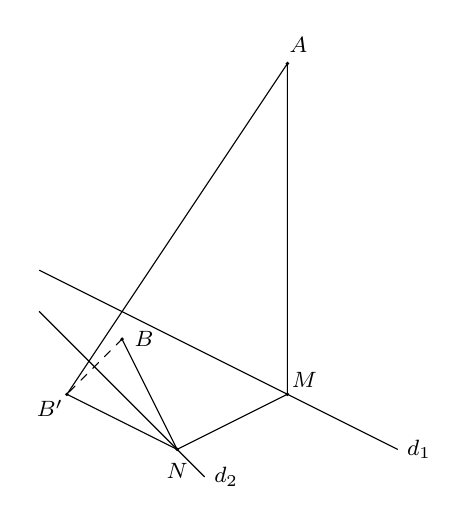
\begin{tikzpicture}[line join=round,line cap=round,font=\footnotesize,scale=0.7,>=stealth]
					 \path
						(1,6)  coordinate (A)
						(-2,1)  coordinate (B)
						(-3,0)  coordinate (B')
						(-1,-1) coordinate  (N)
						(1,0)  coordinate (M);
					\draw[smooth,samples=300,domain=-3.5:3] plot (\x,{-0.5*(\x)+0.5})  node[right]{$d_1$};
					\draw[smooth,samples=300,domain=-3.5:-0.5] plot (\x,{-(\x)-2})  node[right]{$d_2$};
					 \draw (B')--(A)
						 (B')--(N)--(B)
						 (N)--(M)--(A);
					 \draw[dashed](B)--(B');
					\foreach \x/\g in  {A/60,B/0,B'/220,N/-90,M/40}\fill[black] (\x) circle (1pt)+(\g:.4) node{$\x$};
				\end{tikzpicture}
		\end{center}
		Gọi  $B'$ là điểm đối xứng với $B$ qua $d_2$.\\
		Gọi $d$ là đường thẳng qua $B$ và vuông  góc với $d_2\colon \heva{&x=-4+t\\&y=2-t}\Leftrightarrow x+y+2=0$.\\
		Suy ra phương trình của $d$ có dạng $d\colon x-y+m=0$.\\ 
		 Vì $B(-2;1)\in d\Rightarrow-2-1+m=0\Leftrightarrow m=3$. Phương trình của $d$ là $d\colon x-y+3=0$.\\ Gọi $H=d\cap d_2$. Tọa độ của $H$ là nghiệm của hệ
		 $\heva{&x+y+2=0\\&x-y+3=0}\Leftrightarrow \heva{&x=-\dfrac{5}{2}\\&y=\dfrac{1}{2}}\Rightarrow H\left(-\dfrac{5}{2};\dfrac{1}{2}\right)$.\\
		$H$ là trung điểm của $BB'$. Suy  ra\\
		$$\heva{&\dfrac{x_B+x_{B'}}{2}=x_H\\&\dfrac{y_B+y_{B'}}{2}=y_H}\Leftrightarrow \heva{&x_{B'}=2x_H-x_B=2\cdot\left(-\dfrac{5}{2}\right)+2=-3\\&y_{B'}=2y_H-y_B=2\cdot\dfrac{1}{2}-1=0}\Rightarrow  B'(-3;0).$$
		Ta  có $T=AM+BN+MN=AM+B'N+MN\ge AB'=\sqrt{(-3-1)^2+(0-6)^2}=2\sqrt{13}$.\\
		 Đẳng thức xảy ra khi $A$, $M$, $N$, $B'$ thẳng hàng.\\
		Vậy $T_{\min}=2\sqrt{13}\approx  7,21$.
	} 
\end{bt}


%%%%%%%%%%%%%%%% TỰ LUẬN %%%%%%%%%%%%%%%%

% nguồn: MaHoaNH_TuLuan_Lop10
\begin{bt}%[0H9H3-5]%[ma:f7269c39]
	Trong mặt phẳng toạ độ $Oxy$, cho các đường thẳng $d_1\colon x+2y+3=0$, $d_2\colon 3x-y+5=0$ và điểm $P(-2;1)$. Đường thẳng $\Delta$ đi qua $P$ và cắt $d_1, d_2$ lần lượt  tại $A$, $B$ sao cho $P$ là trung điểm của $AB$. Biết khoảng cách từ $M(3;-2)$ đến đường thẳng $\Delta$ có dạng $a\sqrt{b}$. Tính $a^2+b$.
	 \loigiai{
		 Vì $A\in d_1, B\in d_2$ nên giả sử $A(-2t-3;t),B\ (s;3s+5)$.\\
		Ta có $P(-2;1)$  là trung điểm $AB$ nên
		$\heva{&{\dfrac{-2t-3+s}{2}=-2}\\&{\dfrac{t+3s+5}{2}=1}}\Leftrightarrow  \heva{&{-2t+s=-1} \\&{t+3s=-3}}\Leftrightarrow \heva{&{t=0} \\&{s=-1}.}$\\
		 Suy ra $A(-3;0),B(-1;2)$.\\
		Phương trình đường thẳng $\Delta$ đi qua hai điểm $A,B$ là $$\dfrac{x+3}{2}=\dfrac{y}{2} \Leftrightarrow x-y+3=0.$$ Vậy khoảng cách từ $M$ đến đường  thẳng $\Delta$ là $$\mathrm{d}(M,d)=\dfrac{|3-(-2)+3|}{\sqrt{1^2+(-1)^2}}=\dfrac{8}{\sqrt{2}}=4\sqrt{2}.$$
	Suy  ra, $a=4$ và $b=2$ nên $a^2+b=4^2+2=18$.}
\end{bt}

% nguồn: MaHoaNH_TuLuan_Lop10
\begin{bt}%[0H9V3-5]%[ma:fe647ec4]
	Trong mặt phẳng $Oxy$, cho đường thẳng $\Delta\colon a x+b y+c=0$ ($a$; $b$; $c \in \mathbb{N}$; $a \leq 4$) vuông góc với đường thẳng $d\colon 3x-y+4=0$ và $\Delta$ cách $A(1; 2)$ một  khoảng $\sqrt{10}$. Xác định $T=a+b+c$.
	 \loigiai{
		Ta có  $\Delta \perp d \Rightarrow \Delta\colon x+3y+m=0$.
		Theo  đề, ta có
		$$\mathrm{d}(A; \Delta)=\sqrt{10} \Leftrightarrow \dfrac{|7+m|}{\sqrt{10}}=\sqrt{10}  \Leftrightarrow|7+m|=10\Leftrightarrow\hoac{&m=3\\&m=-17.}$$
		Vậy $\Delta_1\colon 3x+4y+3=0$;  $\Delta_2\colon 3x+4y-17=0$.\\
		Vì ($a$; $b$; $c \in \mathbb{N}$;  $a \leq 4$) nên $a=3$; $b=4$; $c=3$. Do đó, $T=10$.
	 }
\end{bt}

% nguồn: MaHoaNH_TuLuan_Lop10
\begin{bt}%[0H9V3-5]%[ma:a1825112]
	Có hai con tàu $A, B$ xuất phát tại bến, chuyển động theo đường thẳng ngoài biển. Trên màn hình ra-đa của trạm điều khiển (xem như mặt phẳng tọa độ $O x y$ với đơn vị trên cả trục tính bằng ki-lô-mét), tại thời điểm $t$  (giờ),
	vị trí của tàu $A$ có tọa độ  được xác định bởi công thức $\heva{ x & = 3 - 3t \\ y & = -4 + 2t }$, vị trí của tàu $B$ có tọa độ là $(4 - 30t; 3 - 40t)$. Nếu tàu $A$ đứng yên ở vị trí ban đầu, tàu $B$ chạy thì khoảng cách gần nhất giữa hai tàu bằng bao nhiêu?
	 \loigiai{
		Với tàu $A$ dừng yên ở vị trí ban đầu nên  tọa độ tàu $A$ luôn ở $t = 0$, suy ra $A(3; -4)$. \\
		Khoảng cách gần nhất giữa hai tàu  là khoảng cách từ điểm $A$ đến đường đi của tàu $B$. \\
		Vì vị trí tàu $B$ có tọa độ là $(4 - 30t; 3 - 40t)$ nên tọa độ tàu $B$ nằm trên đường thẳng $\Delta$ đi qua điểm $M(4; 3)$ và có phương vectơ chỉ phương là $\overrightarrow{u} = (-30;  -40)$.\\
		Do đó đường thẳng $\Delta$ có một vectơ pháp tuyến là $\overrightarrow{n} = (4; -3)$.\\ 
		Phương  trình tổng quát của đường thẳng $\Delta$ là
		$4(x - 4) - 3(y - 3) = 0 \Leftrightarrow 4x  - 3y - 7 = 0$. \\
		Vậy khoảng cách gần nhất giữa hai tàu là $\mathrm{d}(A, \Delta) = \dfrac{|4 \cdot 3 - 3 \cdot (-4) - 7|}{\sqrt{4^2  + (-3)^2}} = \dfrac{17}{5} = 3{,}4$ (km).
	 }
\end{bt}

% nguồn: MaHoaNH_TuLuan_Lop10
\begin{bt}%[0H9V3-5]%[ma:cb682457]
	Cho đường thẳng $\Delta_m\colon (m-2)x+(m+1)y-5m+1=0$ với $m$ là tham  số và điểm $A(-3;9)$. Giả sử $m=\dfrac{a}{b}$ (là phân số tối giản) để khoảng cách từ $A$ đến đường thẳng thẳng $\Delta_m$ là lớn nhất. Khi đó hãy tính giá trị của biểu thức $S=2a-b$.
	 \loigiai{
		Ta  có $\Delta_m\colon (m-2)x+(m+1)y-5m+1=0\Leftrightarrow m(x+y-5)+(-2x+y+1)=0$.\\
		Khi  đó, $\Delta_m$ luôn đi qua điểm cố định $M(2;3)$.\\
		Gọi $AH=\mathrm{d}(A;\Delta_m)=d$ với $H\in \Delta_m$.\\ 
		 Suy ra $d\le AM$.\\
		Do đó $d$ lớn nhất khi $H\equiv M$ hay $M$ là hình  chiếu của $A$ trên $\Delta$.\\
		Ta có $\vec{AM}=(5;-6)$ và  $\Delta_m$ có vecto chỉ phương $\vec{u}(m+1;2-m)$.\\
		Đường thẳng $AM\perp  \Delta_m\Leftrightarrow \vec{AM}\cdot \vec{u}=0$\\
		$\Leftrightarrow 5(m+1)-6(2-m)=0\Leftrightarrow  11m-7=0\Leftrightarrow m=\dfrac{7}{11}$.\\
		Suy ra $S=2a-b=2\cdot 7-11=3$. 
	 }
\end{bt}

% nguồn: MaHoaNH_TuLuan_Lop10
\begin{bt}%[0H9C3-5]%[ma:b451ecb7]
	Cho đường thẳng $\Delta_m\colon (m-2) x+(m+1) y-5m+1=0$ với $m$ là tham số, và điểm $A(-3; 9)$. Giả sử $m=\dfrac{a}{b}$ (là phân số tối giản) để  khoảng cách từ $A$ đến đường thẳng $\Delta_m$ là lớn nhất. Khi đó hãy tính giá trị của biểu thức $S=2a-b$.
	 \loigiai{
		Ta  có $\Delta_m\colon (m-2) x+(m+1) y-5m+1=0\Leftrightarrow m(x+y-5)+(-2x+y+1)=0$.\\
		Điểm  cố định $M(x_0;y_0)$ của $\Delta_m$ có tọa độ thỏa mãn $\heva{&x_0+y_0-5=0 \\&-2x_0+y_0+1=0}\Leftrightarrow\heva{&x_0=2 \\&y_0=3.}$\\
		Gọi $H\in \Delta_m$ là hình chiếu của $A$ trên $\Delta_m$. Khi đó, $\mathrm{d}\left(A, \Delta_m\right)=AH\leq AM$. Do đó $\mathrm{d}\left(A, \Delta_m\right)$ lớn nhất khi $H\equiv M$ hay $M$ là  hình chiếu của $A$ trên $\Delta_m$, tức là $AM\perp \Delta_m$.\\
		Ta có $\overrightarrow{AM}(5;-6)$ và vectơ chỉ phương của $\Delta_m$ là $\overrightarrow{u}=(m+1; 2-m)$. Khi  đó,
		$$AM\perp \Delta_m\Leftrightarrow\overrightarrow{AM}\cdot\overrightarrow{u}=0\Leftrightarrow5(m+1)-6(2-m)=0\Leftrightarrow 11m-7=0\Leftrightarrow  m=\dfrac{7}{11}.$$
		Vậy $S=2a-b=2\cdot7-11=3$. 
	 }
\end{bt}

% nguồn: MaHoaNH_TuLuan_Lop10
\begin{bt}%[0H9K3-5]%[ma:c7df0ee5]
	Trong mặt phẳng $Oxy$ cho đường tròn $(C)\colon x^2+y^2-2x+4 y-4=0$. Viết  phương trình đường thẳng $\Delta$ song song với đường thẳng $d\colon 2 x-y+1=0$ và cắt đường tròn $(C)$ theo một dây cung có độ dài bằng $4$.
	 \loigiai{
	 \immini
		{ 
		Gọi $AB=\Delta \cap (C)$  và $H$ là trung điểm $AB$.\\
		Đường tròn $(C)$ có tâm $I(1;-2)$, bán  kính $R=\sqrt{9}=3$.\\
		Đường thẳng $\Delta$ song song  với $d\colon 2 x-y+1=0$ suy ra $\Delta$ có dạng $$\Delta\colon 2x-y+m=0, (m \neq 1).$$
		Khoảng cách từ $I$ đến  $\Delta$ là $IH=\dfrac{|m+4|}{\sqrt{5}}$.\\
		Xét $\triangle IHA$ vuông tại  $H$, ta có $IH^2=IA^2-AH^2=9-4=5$.
		} 
		{ 
		\begin{tikzpicture}[scale=.75,font=\footnotesize,line join=round,line cap=round,>=stealth]
				\draw (0,0) circle (2cm); 
				\coordinate  (A) at ($(0,0)+(-135:2cm)$);
				\coordinate  (B) at ($(0,0)+(-45:2cm)$);
				 \fill (A) circle (1pt) node[left]{$A$};
				\fill (B) circle  (1pt) node[right]{$B$};
				\fill (0,0)  coordinate (I) circle (1pt) node[above]{$I$};
				\draw  (A)--(B)
					(I)--++(-90:1.41) coordinate  (H) circle (1pt) node[below]{$H$};
				 \def\t{.2}\draw (H)--++(90:\t)--++(180:\t)--++(-90:\t);
			\end{tikzpicture}
		 }\noindent
		 Suy ra
		 $$\dfrac{\left( m+4\right)^2}{5}=5\Leftrightarrow m^2+8m-9=0 \Rightarrow \hoac{& m=1 &\text{(loại)}\\& m=9 &\text{(nhận).}}$$
		Vậy  $\Delta \colon 2x-y+9=0$.
	} 
\end{bt}
